\begin{figure}
	\begin{comment}
	r=9;
	ps=[0.5, 2, 2.3, 2.5, 3.5, 4.5, 6, 8.5];
	eps=1;
	v=3;
	function gen(ps, r, v, eps){
		var dvr = Math.abs(v-r); var s = "";
		ps.push(v);ps.sort();
		var pid = Array.apply(null, Array(ps.length)).map(function (_, i) {return i;})
		pid.sort(function(a, b){var A = Math.abs(ps[a] - r); var B = Math.abs(ps[b] - r); return A>=B ? (A>B?1:0) : -1;});
		ps.sort(function(a, b){var A = Math.abs(a - r); var B = Math.abs(b - r); return A>=B ? (A>B?1:0) : -1;});
		s+=""; for(p in pid){s+=" & $ w_" + pid[p] + " $"}; s+=" \\\\ \\hline\n";
		s+="$ d(w, r) $"; for(p in ps){s+=" & " + Math.abs(ps[p] - r);}; s+=" \\\\ \\hline\n";
		s+="$ x $"; for(p in ps){s+=" & " + ps[p];}; s+=" \\\\ \\hline\n";
		s+="$ \\abs{d(v, r) - d(w, r)} $"; for(p in ps){s+=" & " + Math.abs(dvr - Math.abs(ps[p] - r));}; s+=" \\\\ \\hline\n";
		s+="$ d(w, v) $"; for(p in ps){s+=" & " + Math.abs(ps[p]-v);};s+=" \\\\ \\hline"
		return s;}
	gen(ps, r, v, eps);
	\end{comment}

	\begin{minipage}{\linewidth}
		\centering
		\begin{tikzpicture}
			\draw[thick,->] (0,0) -- (10,0);
			\foreach \x in {0,...,9} {
				\draw (\x cm,1pt) -- (\x cm,-1pt) node[anchor=north] {$\x$};
			}
			
			\newcounter{myCnt}
			\foreach \x in {1, 2.5, 3, 3.5, 4.5, 6, 7, 8, 8.5} {
				\fill(\x,0) circle (3pt);
				\node at (\x,8pt) {$ w_\arabic{myCnt} $};
				\stepcounter{myCnt}
			}
			\fill[blue!25] (3,0) circle (3pt);
			\fill[red] (5,0) circle (3pt);
			
			\node at (5,8pt) {$ r $};
			\node at (10,-8pt) {$ x $};
		\end{tikzpicture}
	
		\begin{tabular}{ | c | c | >{\columncolor{yellow!25}} c | >{\columncolor{yellow!25}} c | >{\columncolor{yellow!25}} c | >{\columncolor{blue!25}} c | >{\columncolor{yellow!25}} c | >{\columncolor{yellow!25}} c | c | c | }
			
			\hline
			& $ w_4 $ & $ w_5 $ & $ w_3 $ & $ w_2 $ & $ w_6 $ & $ w_1 $ & $ w_7 $ & $ w_8 $ & $ w_0 $ \\ \hline
			$ d(w, r) $ & 0.5 & 1 & 1.5 & 2 & 2 & 2.5 & 3 & 3.5 & 4 \\ \hline
			$ x $ & 4.5 & 6 & 3.5 & 3 & 7 & 2.5 & 8 & 8.5 & 1 \\ \hline
			$ \abs{d(v, r) - d(w, r)} $ & 1.5 & 1 & 0.5 & 0 & 0 & 0.5 & 1 & 1.5 & 2 \\ \hline
			$ d(w, v) $ & 1.5 & 3 & 0.5 & 0 & 4 & 0.5 & 5 & 5.5 & 2 \\ \hline
		\end{tabular}
		\subcaption{}\label{odc:tidbscan:linear}
	\end{minipage}
	\linebreak
	\linebreak
	\begin{minipage}{\linewidth}
		\centering
		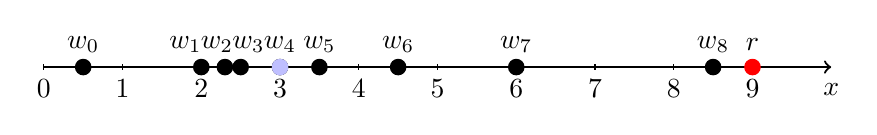
\begin{tikzpicture}
		\draw[thick,->] (0,0) -- (10,0);
		\foreach \x in {0,...,9} {
			\draw (\x cm,1pt) -- (\x cm,-1pt) node[anchor=north] {$\x$};
		}
		
		\setcounter{myCnt}{0}
		
		\fill(0.5,0) circle (3pt);\node at (0.5,8pt) {$ w_\arabic{myCnt} $};\stepcounter{myCnt}
		\fill(2,0) circle (3pt);\node at (1.8,8pt) {$ w_\arabic{myCnt} $};\stepcounter{myCnt}
		\fill(2.3,0) circle (3pt);\node at (2.2,8pt) {$ w_\arabic{myCnt} $};\stepcounter{myCnt}
		\fill(2.5,0) circle (3pt);\node at (2.6,8pt) {$ w_\arabic{myCnt} $};\stepcounter{myCnt}
		% 0.5, 2, 2.3, 2.5, 3.5, 4.5, 6, 8.5
		\foreach \x in {3, 3.5, 4.5, 6, 8.5} {
			\fill(\x,0) circle (3pt);
			\node at (\x,8pt) {$ w_\arabic{myCnt} $};
			\stepcounter{myCnt}
		}
		\fill[blue!25] (3,0) circle (3pt);
		\fill[red] (9,0) circle (3pt);
		
		\node at (9,8pt) {$ r $};
		\node at (10,-8pt) {$ x $};
		\end{tikzpicture}
		\begin{tabular}{ | c | c | c | c | >{\columncolor{yellow!25}} c | >{\columncolor{blue!25}} c | >{\columncolor{yellow!25}} c | >{\columncolor{yellow!25}} c | >{\columncolor{yellow!25}} c | c | }
			\hline                                                                                                       
			& $ w_8 $ & $ w_7 $ & $ w_6 $ & $ w_5 $ & $ w_4 $ & $ w_3 $ & $ w_2 $ & $ w_1 $ & $ w_0 $ \\ \hline
			$ d(w, r) $ & 0.5 & 3 & 4.5 & 5.5 & 6 & 6.5 & 6.7 & 7 & 8.5 \\ \hline
			$ x $ & 8.5 & 6 & 4.5 & 3.5 & 3 & 2.5 & 2.3 & 2 & 0.5 \\ \hline
			$ \abs{d(v, r) - d(w, r)} $ & 5.5 & 3 & 1.5 & 0.5 & 0 & 0.5 & 0.7 & 1 & 2.5 \\ \hline
			$ d(w, v) $ & 5.5 & 3 & 1.5 & 0.5 & 0 & 0.5 & 0.7 & 1 & 2.5 \\ \hline
		\end{tabular}
		\subcaption{}\label{odc:tidbscan:log}
	\end{minipage}
	\caption{Znajdowanie otoczenia $ \varepsilon=1 $ punktu $ v=3 $ w jednowymiarowym zbiorze danych przy pomocy nierówności trójkąta z punktem referencyjnym $ r $.}
\end{figure}
